% !TeX encoding = UTF-8

%% ------------------------------------------------------------------------
%% Copyright (C) 2021,2022 SJTUG
%% 
%% SJTUBeamer Example Document by SJTUG
%% 
%% SJTUBeamer Example Document is licensed under a
%% Creative Commons Attribution-NonCommercial-ShareAlike 4.0 International License.
%% 
%% You should have received a copy of the license along with this
%% work. If not, see <http://creativecommons.org/licenses/by-nc-sa/4.0/>.
%%
%% For a quick start, check out src/doc/sjtubeamerquickstart.tex
%% Join discussions: https://github.com/sjtug/SJTUBeamer/discussions
%% -----------------------------------------------------------------------

\documentclass[xcolor=table,dvipsnames,svgnames,aspectratio=169]{ctexbeamer}
% 可以通过 fontset=macnew / fontset=ubuntu / fontset=windows 选项切换字体集

\usepackage{tikz}
\usepackage[normalem]{ulem}
\usetikzlibrary{arrows}
\usepackage{amsmath}
\usepackage{mflogo}
\usepackage{graphicx}
\usepackage{ccicons}
\usepackage{hologo}
\usepackage{colortbl}
\usepackage{shapepar}
\usepackage{hyperxmp}
\usepackage{booktabs}
\usepackage{qrcode}
\usepackage{listings}
\usepackage{tipa}
\usepackage{multicol}
\usepackage{datetime2}
\usepackage{fontawesome5}
\usepackage{hyperref}

% 参考文献设置,使用 style=gb7714-2015 样式为标准顺序编码制,
% 使用 style=gb7714-2015ay 样式可以改为著者-出版年制。
\usepackage[backend=biber,style=gb7714-2015]{biblatex}
\addbibresource{thesis.bib}

\graphicspath{{figures/}}

% 不可以出现 Logo 的!
\setbeamertemplate{logo}{}
% \logo{logo.png}
\logo{}

\hypersetup{
  % pdfsubject = {上海交通大学图书馆专题培训讲座},
  % pdfauthor = {Alexara Wu},
  % pdfcopyright = {Licensed under CC-BY-SA 4.0. Some rights reserved.},
  % pdflicenseurl = {http://creativecommons.org/licenses/by-sa/4.0/},
  unicode = true,
  psdextra = true,
  pdfdisplaydoctitle = true
}

\pdfstringdefDisableCommands{
  \let\\\relax
  \let\quad\relax
  \let\hspace\@gobble
}

\renewcommand{\TeX}{\hologo{TeX}}
\renewcommand{\LaTeX}{\hologo{LaTeX}}
\newcommand{\BibTeX}{\hologo{BibTeX}}
\newcommand{\XeTeX}{\hologo{XeTeX}}
\newcommand{\pdfTeX}{\hologo{pdfTeX}}
\newcommand{\LuaTeX}{\hologo{LuaTeX}}
\newcommand{\MiKTeX}{\hologo{MiKTeX}}
\newcommand{\MacTeX}{Mac\hologo{TeX}}
\newcommand{\beamer}{\textsc{beamer}}
\newcommand{\XeLaTeX}{\hologo{Xe}\kern-.13em\LaTeX{}}
\newcommand{\pdfLaTeX}{pdf\LaTeX{}}
\newcommand{\LuaLaTeX}{Lua\LaTeX{}}

\def\TeXLive{\TeX{} Live}
\let\TL=\TeXLive
\newcommand{\SJTUThesis}{\textsc{SJTUThesis}}
\newcommand{\SJTUThesisVersion}{1.1.0}
\newcommand{\SJTUThesisDate}{2022/3/26}
\newcommand{\SJTUBeamer}{\textsc{SJTUBeamer}}
\newcommand{\SJTUBeamerVersion}{3.0.0}
\newcommand{\SJTUBeamerDate}{2022/11/22}

\newcommand\link[1]{\href{#1}{\faLink}}
\newcommand\pkg[1]{\texttt{#1}}

\def\cmd#1{\texttt{\color{structure}\footnotesize $\backslash$#1}}
\def\env#1{\texttt{\color{structure}\footnotesize #1}}
\def\cmdxmp#1#2#3{\small{\texttt{\color{structure}$\backslash$#1}\{#2\}
\hspace{1em}\\ $\Rightarrow$\hspace{1em} {#3}\par\vskip1em}}

\lstset{
  language=[LaTeX]TeX,
  basicstyle=\ttfamily\footnotesize,
  tabsize=2,
  keywordstyle=\bfseries\ttfamily\color{cprimary},
  commentstyle=\sl\ttfamily\color[RGB]{100,100,100},
  stringstyle=\ttfamily\color[RGB]{50,50,50},
  extendedchars=true,
  breaklines=true,
}

\usetheme[maxplus]{sjtubeamer}
% 使用 maxplus/max/min 切换标题页样式
% 使用 red/blue 切换主色调
% 使用 light/dark 切换亮/暗色模式
% 使用外样式关键词以获得不同的边栏样式
%   miniframes infolines  sidebar
%   default    smoothbars split	 
%   shadow     tree       smoothtree
% 使用 topright/bottomright 切换徽标位置
% 使用逗号分隔列表以同时使用多种选项

% \tikzexternalize[prefix=build/]
% 如果您需要缓存 tikz 图像,请取消注释上一行,并在编译选项中添加 -shell-escape。

\author{某同学}
\institute[SUEP]{2021391}
\date{\the\year 年 \the\month 月}
% \subject{LaTeX, 论文排版, SJTUThesis}

\title[人工智能在模拟CMOS电路设计中的应用与展望] % 页脚显示标题
{\textbf{人工智能在模拟CMOS电路设计中的应用与展望}} % 首页标题

\begin{document}

% 使用节目录
\AtBeginSection[]{
  \begin{frame}
    %% 使用传统节目录,也可以将 subsectionstyle=... 换成 hideallsubsections 以隐藏所有小节信息
    \tableofcontents[currentsection,subsectionstyle=show/show/hide]
    %% 或者使用节页
    % \sectionpage
  \end{frame}
}

% 使用小节目录
\AtBeginSubsection[]{		       % 在每小节开始
  \begin{frame}
    %% 使用传统小节目录
    \tableofcontents[currentsection,subsectionstyle=show/shaded/hide]
    %% 或者使用小节页
    % \subsectionpage
  \end{frame}
}

\maketitle

% \begin{frame}{目录}
%   \tableofcontents[hideallsubsections]	% 隐藏所有小节信息
% \end{frame}

% 引言与选题意义
\begin{frame}{引言与选题意义}
  \begin{itemize}
      \item 模拟CMOS电路在通信、医疗和消费电子中扮演重要角色。
      \item 传统设计周期长、成本高,而AI能大幅优化这一过程。
      \item 探索AI在电路设计中的应用,为产业带来变革。
  \end{itemize}
  \begin{center}
      % \includegraphics[width=0.7\textwidth]{importance.png} % 建议:展示传统设计与AI设计的对比
  \end{center}
\end{frame}

% AI在CMOS电路设计中的主要应用
\begin{frame}{AI在CMOS电路设计中的主要应用}
  \begin{enumerate}
      \item 自动化设计流程
      \item 性能优化(功耗、增益、带宽等)
      \item 电路验证与测试
      \item 设计迁移(新工艺节点)
  \end{enumerate}
  \begin{center}
      % \includegraphics[width=0.7\textwidth]{applications.png} % 建议:展示AI在EDA流程中的应用示意图
  \end{center}
\end{frame}

% 强化学习在电路设计中的应用
\begin{frame}{强化学习在电路设计中的应用}
  \begin{itemize}
      \item RL在复杂设计空间中进行探索,快速找到最优解。
      \item 助力参数优化,如芯片布局、晶体管尺寸调整等。
      \item 挑战:训练时间长、收敛速度慢。
  \end{itemize}
  \begin{center}
      % \includegraphics[width=0.7\textwidth]{RL_example.png} % 建议:展示强化学习在芯片设计中的实际案例
  \end{center}
\end{frame}

% 深度神经网络(DNN)提升设计效率
\begin{frame}{深度神经网络(DNN)提升设计效率}
  \begin{itemize}
      \item DNN可预测电路性能,减少仿真次数。
      \item 示例:BagNet 框架实现 200 倍效率提升。
      \item 未来:进一步提升智能化设计能力。
  \end{itemize}
  \begin{center}
      % \includegraphics[width=0.7\textwidth]{DNN_performance.png} % 建议:展示DNN用于性能预测的示意图
  \end{center}
\end{frame}

% AI在工艺节点迁移中的应用
\begin{frame}{AI在工艺节点迁移中的应用}
  \begin{itemize}
      \item AI自动适应新工艺节点,实现设计迁移。
      \item 案例:三星从14nm迁移到5nm节点,用AI完成布局优化。
      \item 产品上市时间大幅缩短。
  \end{itemize}
  \begin{center}
      % \includegraphics[width=0.7\textwidth]{node_migration.png} % 建议:展示节点迁移的流程图
      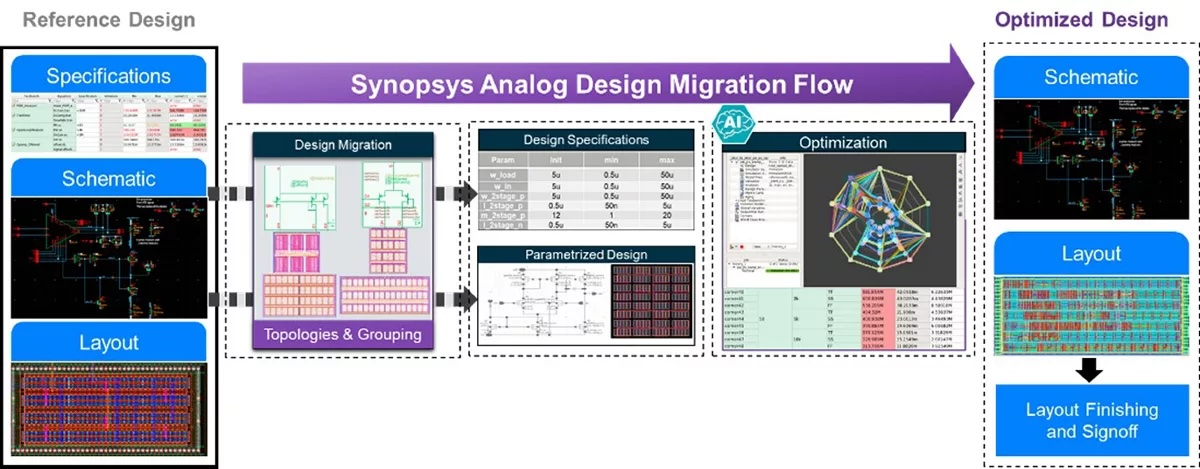
\includegraphics[width=0.5\textwidth]{figure-2-3-analog-design-migration-flow.jpg} 
  \end{center}
\end{frame}

% 国内外研究进展
\begin{frame}{国内外研究进展}
  \begin{itemize}
      \item 全球公司,如三星、台积电和英特尔,推动AI在EDA中的应用。
      \item 国内的华为和清华大学也在开发智能设计工具。
      \item AI将引领未来电路设计的技术变革。
  \end{itemize}
  \begin{center}
      % \includegraphics[width=0.7\textwidth]{global_progress.png} % 建议:展示各公司在AI电路设计中的进展
  \end{center}
\end{frame}

% 挑战与未来展望
\begin{frame}{挑战与未来展望}
  \begin{itemize}
      \item 挑战:高维设计空间复杂性、工具精度需求、流程整合问题。
      \item 未来:优化AI算法,提高设计流程自动化程度。
      \item AI将成为推动电路设计技术进步的重要引擎。
  \end{itemize}
\end{frame}

% 总结
\begin{frame}{总结}
  \begin{itemize}
      \item AI技术在模拟CMOS电路设计中展现了显著优势。
      \item 从自动化设计到工艺迁移,AI大幅提升了设计效率与可靠性。
      \item 未来,AI将继续引领电路设计领域的技术创新。
  \end{itemize}
  \begin{center}
      % \includegraphics[width=0.5\textwidth]{conclusion.png} % 建议:展示总结性图表或文字云
  \end{center}
\end{frame}

\makebottom

\end{document}
